\documentclass[aspectratio=169]{beamer}
\usepackage[utf8]{inputenc} % codificacao de caracteres
\usepackage[T1]{fontenc}    % codificacao de fontes
\usepackage[english]{babel}  % idioma
\usepackage{graphics,amssymb,amsfonts,amsmath}
\usepackage{tikz}
\usepackage{enumerate,hyperref}
\usepackage{palatino}	% Fonte sem serifa
\usepackage{ragged2e}	% Paragrafo justificado
%\usepackage{minted}	% Highlight para codigos de programacao
\usepackage{booktabs} % tabelas
\usepackage{multicol}
\usepackage{multirow}
%\usepackage[table]{xcolor}


% Veja mais temas e cores em http://www.hartwork.org/beamer-theme-matrix/
\usetheme{Montpellier}         % tema
\usecolortheme{orchid}      % cores
\usefonttheme[onlymath]{serif} % fonte modo matematico
% Colocando numero de paginas no slide
\setbeamertemplate{footline}[frame number]



\DeclareGraphicsExtensions{.pdf,.jpg,.png} % compilamos apenas com pdflatex
\graphicspath{{figuras/}} % caminho onde as figuras estarao disponiveis




% ---------------------------------------------------------------------------- %
% T�tulo                                                                       %
% ---------------------------------------------------------------------------- %

\title[\sc{Teoria de Circuitos Eletrônicos 1}]{\LARGE Aula 4 - Exercise Class 1}
\author[Prof. Marcelino Andrade]{Prof. Marcelino Andrade}
\institute{Faculdade UnB Gama} % opcional
\date{\today}

\begin{document}
\justifying % Paragrafo justificado
\pagebreak

\begin{frame}
  \titlepage
\end{frame}


% ----------------- NOVO SLIDE --------------------------------
\begin{frame}{Contents\newline}

\tableofcontents
\begin{center}	
     		Fundamentals of Electric Circuits (Alexander and Sadiku), 4th Edition			
\end{center}	
\end{frame}

% ----------------- NOVA SECÇÂO -----------------------------
\section{Kirchhoff’s Laws (2.4)}
% ----------------- NOVO SLIDE --------------------------------
\begin{frame}[fragile]
	\frametitle{Kirchhoff’s Laws}
\begin{tabular}{ll}
	\begin{columns}
		\begin{column}{1\textwidth}  %%<--- here
		\textbf{Practice Problem 2.7} - Find $v_{0}$ and $i_{0}$ in the circuit.\\
		\begin{center}
    			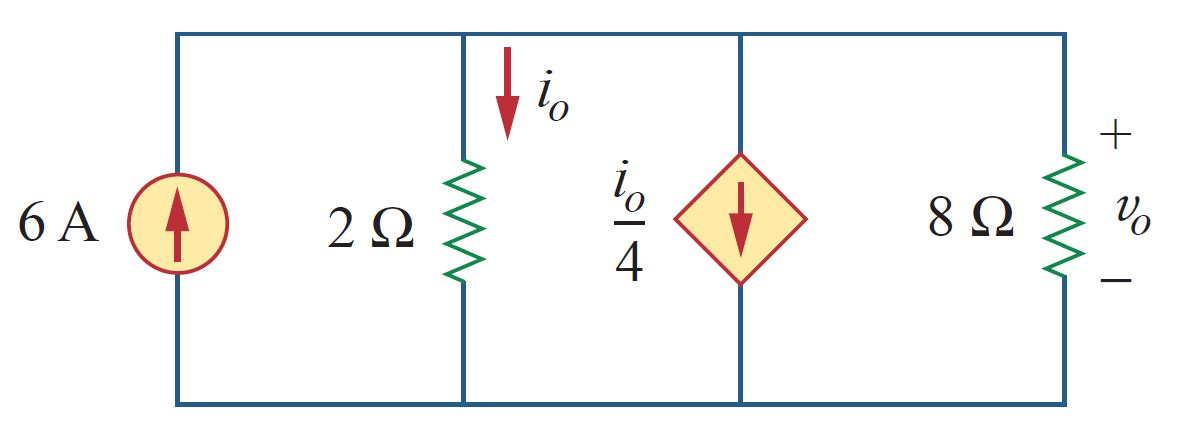
\includegraphics[height=.2\textwidth]{figura1.jpg}	
		\end{center}	
		\scalebox{0.8}{Answer: $i_{0}= 4A \ and \ v_{0}=8V$}
		\end{column}
	\end{columns}
\end{tabular}
\end{frame}
% ----------------- NOVO SLIDE --------------------------------
\begin{frame}[fragile]
	\frametitle{Kirchhoff’s Laws}
\begin{tabular}{ll}
	\begin{columns}
		\begin{column}{1\textwidth}  %%<--- here
		\textbf{Practice Problem 2.8} - Find the currents and voltages in the circuit shown.\\
		\begin{center}
    			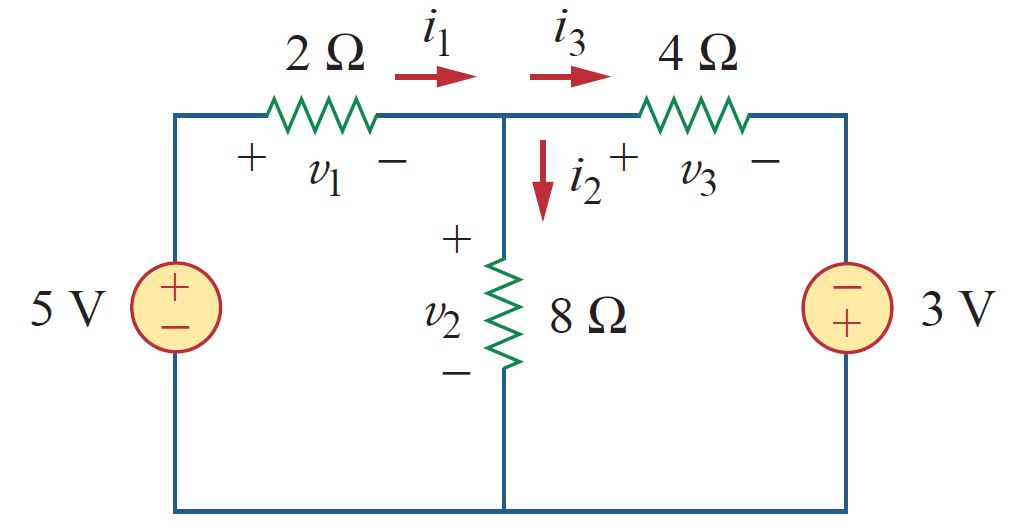
\includegraphics[height=.25\textwidth]{figura2.jpg}	
		\end{center}	
		\scalebox{0.8}{Answer: $v_{1}= 3V, v_{2}=2V, v_{3}=5V, i_{1}=1.5A, i_{2}=0.25A \ and \ i_{3}=1.25V$}
		\end{column}
	\end{columns}
\end{tabular}
\end{frame}
% ----------------- NOVA SECÇÂO -----------------------------
\section{Voltage Division (2.5) and Current Division (2.6)}

\begin{frame}[fragile]

	\frametitle{Voltage Division and Current Division}
\begin{tabular}{ll}
	\begin{columns}
		\begin{column}{1\textwidth}  %%<--- here
		\textbf{Practice Problem 2.12} - Find $v_{1}$ and $v_{2}$ in the circuit shown. Also calculate $i_{1}$ and $i_{2}$ the power dissipated in the $12 \Omega$ and $40\Omega$ resistors.\\
		\begin{center}
    			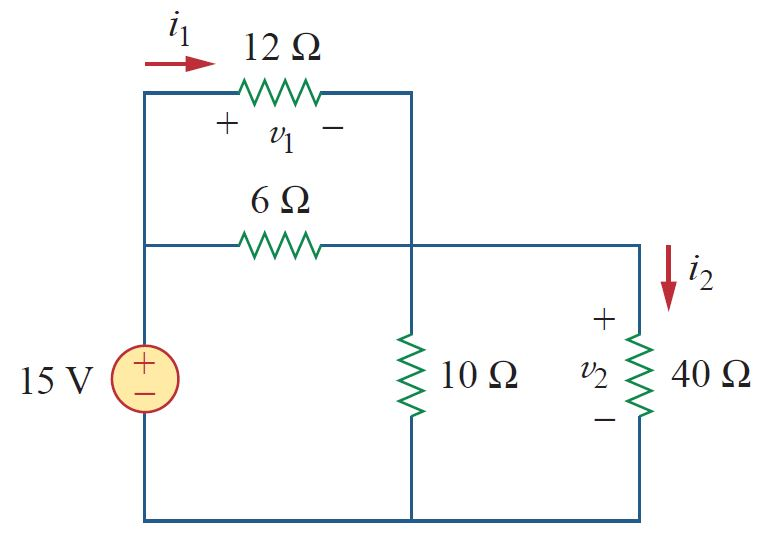
\includegraphics[height=.2\textwidth]{figura3.jpg}	
		\end{center}	
		\scalebox{0.8}{Answer: $v_{1}= 5V, i_{1}=416.7mA, p_{1}=2.083W, v_{2}=10V, i_{2}=250mA \ and \ p_{2}=2.5W$}
		\end{column}
	\end{columns}
\end{tabular}
\end{frame}


% ----------------- NOVA SECÇÂO -----------------------------
\begin{frame}[fragile]

	\frametitle{Equivalent Resistance}
\begin{tabular}{ll}
	\begin{columns}
		\begin{column}{1\textwidth}  %%<--- here
		\textbf{Problem 2.38} - Find $R_{eq}$ and $i_{o}$ in the circuit.\\
		\begin{center}
    			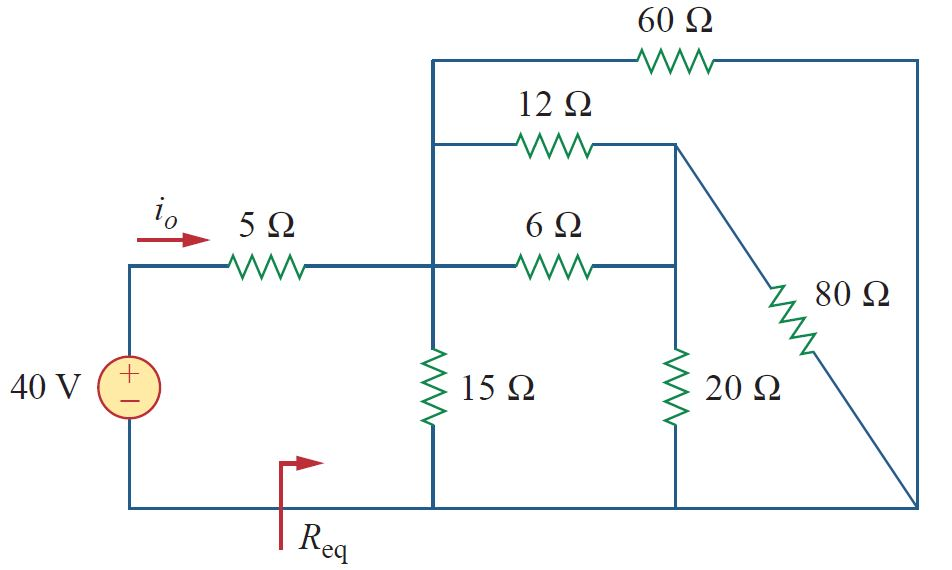
\includegraphics[height=.3\textwidth]{figura4.jpg}	
		\end{center}	
		
		\end{column}
	\end{columns}
\end{tabular}
\end{frame}

% ----------------- NOVA SECÇÂO -----------------------------
\section{Nodal Analysis (3.2)}

\begin{frame}[fragile]

	\frametitle{Nodal Analysis}
\begin{tabular}{ll}
	\begin{columns}
		\begin{column}{1\textwidth}  %%<--- here
		\textbf{Problem 2.25} - For the network, find the current, voltage, and power associated with the 20-k$\Omega$
resistor.\\
		\begin{center}
    			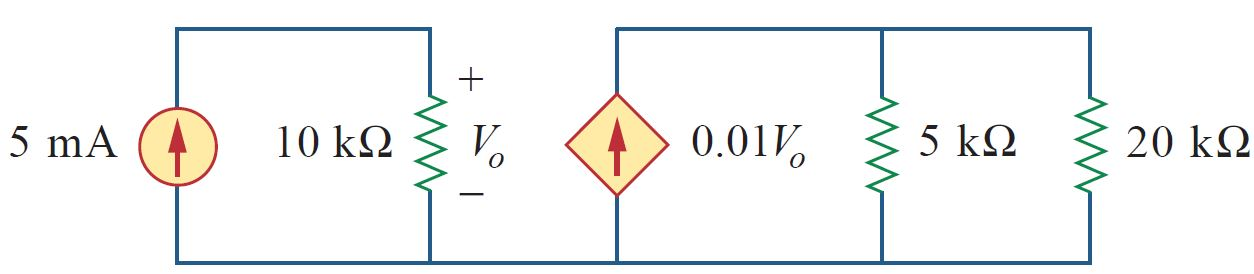
\includegraphics[height=.2\textwidth]{figura5.jpg}	
		\end{center}	
		\scalebox{0.8}{Answer: $i= 0.1A, v=2kV, \ and \  p=0.2kW$}
		\end{column}
	\end{columns}
\end{tabular}
\end{frame}

% ----------------- NOVO SLIDE --------------------------------

\begin{frame}[fragile]

	\frametitle{Nodal Analysis}
\begin{tabular}{ll}
	\begin{columns}
		\begin{column}{1\textwidth}  %%<--- here
		\textbf{Practice Problem 3.2} - Find the voltages at the three nonreference nodes in the circuit.\\
		\begin{center}
    			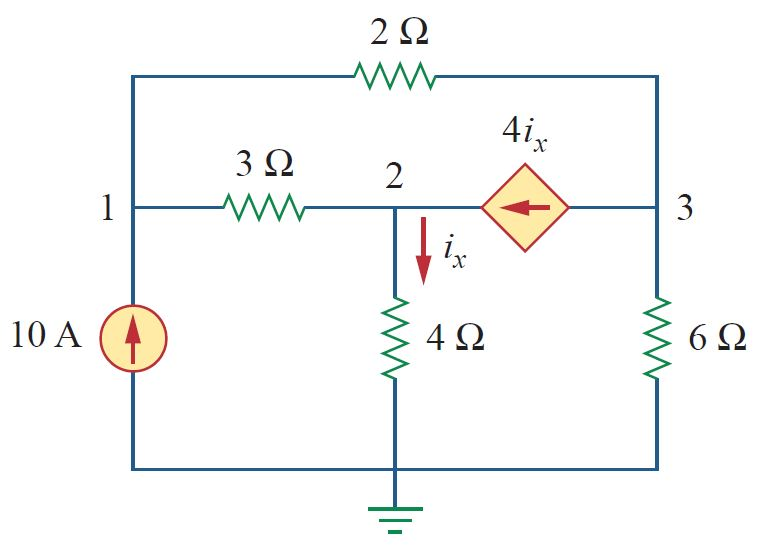
\includegraphics[height=.3\textwidth]{figura6.jpg}	
		\end{center}	
		\scalebox{0.8}{Answer: $v_{1}= 80V, v_{2}=-64V, \ and \  v_{3}=156V$}
		\end{column}
	\end{columns}
\end{tabular}
\end{frame}

% ----------------- NOVO SLIDE --------------------------------
\begin{frame}[fragile]

	\frametitle{Nodal Analysis}
\begin{tabular}{ll}
	\begin{columns}
		\begin{column}{1\textwidth}  %%<--- here
		\textbf{Practice Problem 3.4} - Find $v_{1}$, $v_{2}$ and $v_{3}$ in the circuit using nodal analysis.\\
		\begin{center}
    			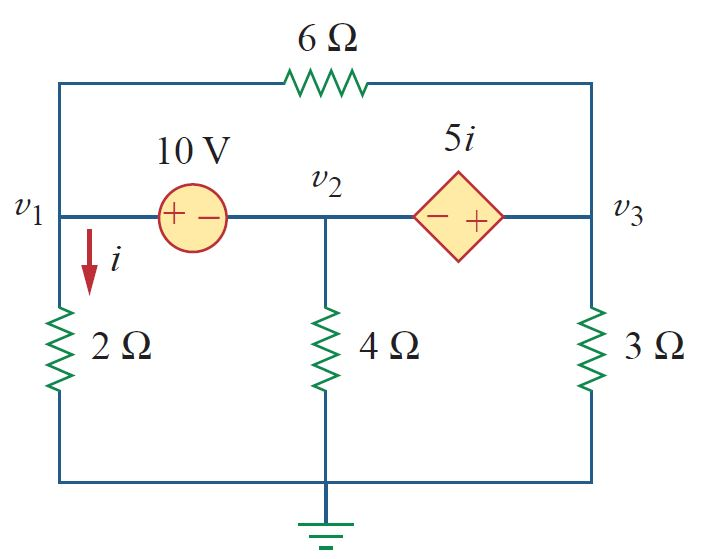
\includegraphics[height=.25\textwidth]{figura7.jpg}	
		\end{center}	
		\scalebox{0.8}{Answer: $v_{1}= 3.043V, v_{2}=-6.956V, \ and \  v_{3}=0.6522V$}
		\end{column}
	\end{columns}
\end{tabular}
\end{frame}


% ----------------- NOVA SECÇÂO -----------------------------
\section{Mesh Analysis (3.4)}
% ----------------- NOVO SLIDE --------------------------------

\begin{frame}[fragile]

	\frametitle{Mesh Analysis}
\begin{tabular}{ll}
	\begin{columns}
		\begin{column}{1\textwidth}  %%<--- here
		\textbf{Practice Problem 3.5} - Calculate the mesh currents and of the circuit.\\
		\begin{center}
    			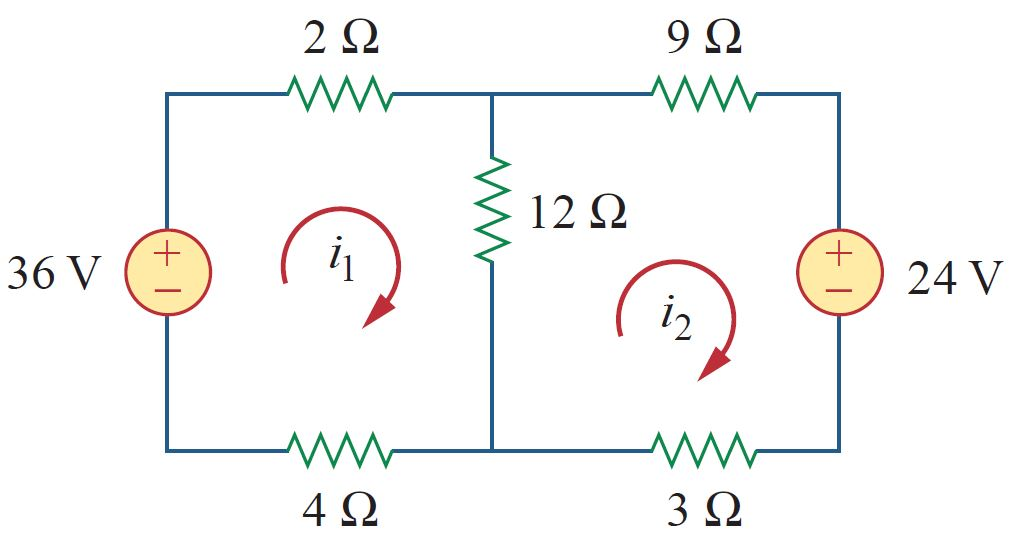
\includegraphics[height=.25\textwidth]{figura8.jpg}	
		\end{center}	
		\scalebox{0.8}{Answer: $i_{1}= 2A \ and \  i_{2}=0A$}
		\end{column}
	\end{columns}
\end{tabular}
\end{frame}
% ----------------- NOVO SLIDE --------------------------------
\begin{frame}[fragile]

	\frametitle{Mesh Analysis}
\begin{tabular}{ll}
	\begin{columns}
		\begin{column}{1\textwidth}  %%<--- here
		\textbf{Practice Problem 3.13} -The transistor circuit has $\beta=80$ and $v_{BE}=0.7V$. Find $v_{0}$ and $i_{0}$.\\
		\begin{center}
    			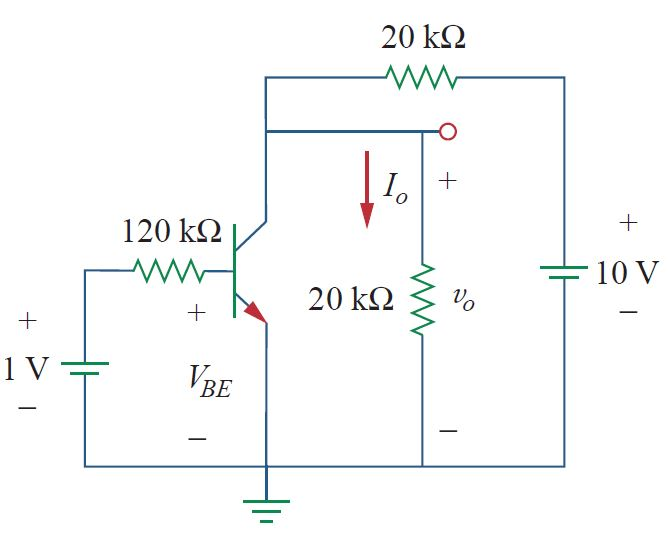
\includegraphics[height=.25\textwidth]{figura9.jpg}	
			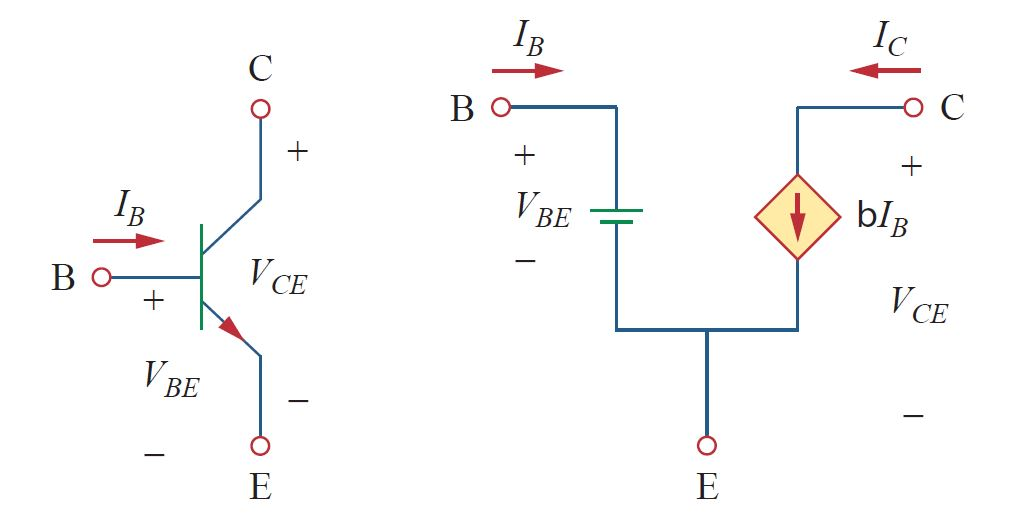
\includegraphics[height=.25\textwidth]{figura10.jpg}
		\end{center}	
		\scalebox{0.8}{Answer: $v_{0}= 3V \ and \  i_{0}=150 \mu A$}
		\end{column}
	\end{columns}
\end{tabular}
\end{frame}
% ----------------- NOVO SLIDE --------------------------------

\begin{frame}[fragile]

	\frametitle{Mesh Analysis}
\begin{tabular}{ll}
	\begin{columns}
		\begin{column}{1\textwidth}  %%<--- here
		\textbf{Problem 3.91} - For the transistor circuit, find $I_{B}$, $V_{CE}$ and $v_{o}$. Take $\beta=200$ and $V_{BE}=0.7 V$.\\
		\begin{center}
    			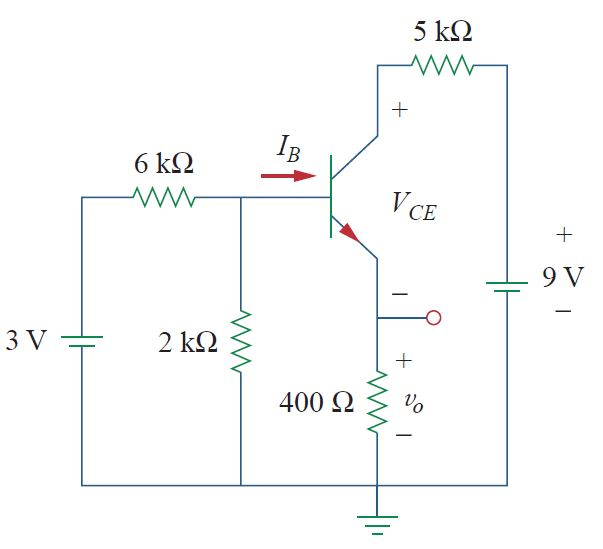
\includegraphics[height=.25\textwidth]{figura11.jpg}	
		\end{center}	
		\scalebox{0.8}{Answer: $v_{B}= 0.61/muA, V_{CE}=8.34V \ and \  v_{0}=49 mA$}
		\end{column}
	\end{columns}
\end{tabular}
\end{frame}











\end{document} 